\documentclass[10pt,twocolumn]{confpaper}

%%%%%%%%%%%%%%%%%%%%  INCLUDES  %%%%%%%%%%%%%%%%%%%%%%%%%%
\usepackage{graphicx} 
\usepackage{caption,subcaption}
% \usepackage[showframe]{geometry}
% \definecolor{darkgreen}{rgb}{0.0, 0.65, 0.0}

\ifthenelse{\equal{\COMMENTS}{no}}{%
\newcommand{\ag}[1]{\textit{\textcolor{blue}{[arpit]: #1}}} % Arpit's comments

}{
\newcommand{\ag}[1]{}

}

\newcommand{\supsym}[1]{\raisebox{4pt}{{\footnotesize #1}}}
\newcommand{\et}{\supsym{$\dag$}}
\newcommand{\ucl}{\supsym{$\diamond$}}
\newcommand{\ptn}{\supsym{$\star$}}
\newcommand{\ceq}{\supsym{$\ddag$}}


\usepackage{listing}



\usepackage{amsmath}
\usepackage{pifont}
\usepackage[linesnumbered, ruled, vlined]{algorithm2e}
\usepackage{fancybox}
\usepackage{pseudocode}
\usepackage{algpseudocode}
\usepackage{booktabs} % For formal tables
\usepackage{outlines}
\usepackage{listings} 
\usepackage{tabularx}
\usepackage{colortbl, graphicx}
\usepackage{subcaption}
\usepackage{balance}
\usepackage{paralist}
\usepackage{tcolorbox}


\usepackage{hyperref}
\hypersetup{
    colorlinks=true,
    linkcolor=blue,
    filecolor=magenta,      
    urlcolor=cyan,
    pdftitle={Overleaf Example},
    pdfpagemode=FullScreen,
    }

\urlstyle{same}

%%%%%%%%%%%%%%%%%%%%  LOCALS  %%%%%%%%%%%%%%%%%%%%%%%%%%%%
% System name macro
\newcommand{\system}{Sonata\xspace}

%%%%%%%%%%%%%%%%%%%%  TITLE/AUTHORS  %%%%%%%%%%%%%%%%%%%%%
\newcommand{\TITLE}{Title}

\date{}
\title{
{CMPSC 190N\\ Classifying Video Content as Gaming or Music using Networking insight}}
\author{
{Yulin Lin Côme Bonal}
}

%%%%%%%%%%%%%%%%%%%%  START OF DOCUMENT  %%%%%%%%%%%%%%%%%

\begin{document}
\maketitle
\thispagestyle{empty}

%\AcmCopyright
%\ToAppear

\begin{sloppypar}

\begin{abstract}
\textit{A good abstract should have the following key components: }
\begin{itemize}
    \item \textbf{Common ground}: \textit{Here, you should specify beliefs, assumptions, etc. that are acceptable to readers as unproblematic. For example, results from prior research that is generally accepted in the community. Any story, anecdote, or incident that is relevant to the paper but represents stability. The purpose of this text is to contextualize what follows, but most importantly, it sets up a situation just so that it can be disrupted. }\hl{Music videos obviously require less bandwidth to load than the gaming ones, furthermore, video games graphics and image quality have significantly increased over the years and are expected to continue advancing, resulting in distinct networking demands.}
    \item \textbf{Disruption}: \textit{Here, you present the destabilizing condition. The destabilizing condition can be errors in prior works/understanding, false assumptions, ignorance, contradictions, etc.}\hl{The first struggle we went through came along with the range of data we were working on, since the provided dataset is limited to mere "videos", we were unable to accurately pick two videos respectively labeled as "gaming" and "audio only". Secondly, we ran into a server issue which prevented us from connecting to the right aws-fargate. Finally, we faced problems with files not updating correctly, as well as permission issues when attempting to modify.}
    \item \textbf{Cost}: \textit{Here, you highlight the cost of destabilizing conditions. What do we lose by sticking with the status quo?} \hl{The consequences of the aforementioned roadblocks we encountered result  in inefficient resource allocation, as resources are wasted on videos that do not require as much resources to play.}
    \item \textbf{Resolution}: \textit{Here, you talk about your approach to solving the problem described above. You provide a gist of your solution, and an intuition on why you think it will work. The intuition can be based on new observations or an overview of results.} \hl{In order to find accurate data we could train our model on, we manually picked two video, one for each category our machine learning model aims to classify. Regarding the server issue, we solved it by trying differents servers / node. Lastly, when it comes to the files problems, we managed the find the correct paths to get rid of this issue.}
\end{itemize}



\end{abstract}






\section{Introduction}
\label{sec:intro}
 



\textbf{Paragraph 1}: Video games and streaming are experiencing advancements in graphics and resolution over the last decades, therefore, it is relevant to ensure if the network traffic classification still works efficiently as it used to. The performed classifications could result as a better allocation of resources allowing us to manage the bandwidth in the most optimal way to avoid wasting it. 


\textbf{Paragraph 2}: Nowadays, the fast growth of online activities such as streaming and gaming puts immense demands on the network infrastructure. Traditional approaches to traffic classification cannot stand up to the complexity and diversity of data flows. Our project aimed to address this challenge by leveraging machine learning to differentiate between gaming and music video traffic coming from the same source (youtube) in order to make networks efficient enough to meet the needs of our time.


\textbf{Paragraph 3}: In this paper, we came up with a new approach to traffic classification, which differentiates between gaming and music video, both sourced from YouTube. By using our own dataset and machine learning techniques, our work introduces a classification method by identifying these distinct traffic types. First, instead of training our model on mock data, we consider the real-world traffic data and, through a pipeline performing the key features one by one, such as packet size / frequency, data spikes. Our findings reveal that differentiating between gaming and music videos is not just about optimizing network resource allocation, it represents an significant step made toward redesigning and modernizing networks to align with the current era we live in. By addressing this gap, our project lays the groundwork for  smarter and more flexible networking solutions in accordance to the digital era.



\textbf{Paragraph 4}: We came across a related study called Beauty and the Burst, which explores the burstiness of network traffic and how it affects traffic characterization and quality of service. The study offers valuable insights into how bursty behavior impacts network performance across a wide range of applications. However, our approach is different. While Beauty and the Burst focuses on the pattern of traffic at a larger scale, our contribution focuses on the classification of gaming and music video traffic over platforms like YouTube. By using machine learning and a custom dataset specifically designed for this purpose, we restrict ourselves to diving deeper into the unique characteristics of these traffic types and exploring ways to optimize resource allocation more effectively. This focused approach highlights the unique contributions of our work.



\textbf{Paragraph 5}: The rest of this paper is organized as follows. The second section give further insights on the project's purpose and which needs it aims to satisfy explaining how relevant it is in the given context. In the third section we will be describing our approach toward the expected result, breaking it down into different stages such as the data collection process and how we plan to handle them. Throughout the section 4, we will dive deeper into the technical details, focusing on the implementation of our machine learning model specifically. The fifth section will be related to our findings, we will be discussing their relevancy as well as we will compare them to the results expected initially, this section will also be devoted to provide any pertinent graph which is related to our work. Lastly, in Section 6, we summarize the essential conclusions of this work, discuss potential challenges faced, and provide thoughtful suggestions for advancing this research in the future.







\section{Background and Motivation}
\label{sec:background}

This is the section where you provide appropriate background to readers who do not have expertise in the specific subfield. You might find some pointers from \href{https://www.seas.upenn.edu/~nyaseen/PaperWriting2.pdf}{Nofel} useful here: 
\begin{itemize}
    \item Precisely specify the problem statement and problem context. 
    \item State all your assumptions, definitions here. Rationalize your assumptions. 
    \item What are the current approaches to solve this problem? 
    \item What are their limitations? If possible, provide an overview of the design space and try to place your approach in this space compared to other solutions. 
    \item Mention any unique observation that motivates your current approach. 
\end{itemize}

Your goal here is to convince the reader that the proposed solution is scoped relative to related work. This section should present an argument why “obvious solutions” (strawman) and competing publications are not effective/applicable with logic, data, or experimental evidence.
\section{Design/Approach/Methodology} 
Here, you want to ensure that your approach/system design is completely described in sufficient detail for the reader to potentially replicate the work. Make sure you motivate all the key ``design decisions'' with logic, data, or experiments.


\label{sec:design}

\hl{This section describes the methodology employed from scratch to overcome the challenges in distinguishing between gaming and music video traffic on YouTube. We designed an approach that incorporates data collection, feature extraction, and model training to achieve accurate and adaptive classification.}

\vspace{2mm}


\hl{The implemented pipeline works as follows :}
\begin{itemize}
    \item \hl{\textbf{Data Collection:} The first step in our methodology involves capturing network traffic data directly from Youtube, we aim to collect traffic traces from both gaming and music video. In order to do so, and to ensure sufficient diversity within our dataset, we collected approximately 2000 seconds of data by recording 18 videos for training and 2 videos for testing, each with 100 seconds of traffic data. This process resulted in around 15,000 rows of data for analysis.}
    \item \hl{\textbf{Traffic Capture:} We log raw network traffic into two\texttt{.pcap} files respectively for the two categories we are trying to distinguish, as the pipeline is streaming the videos. This captures essential data such as packet size and frequency or any other data that would be useful to help our model labeling videos.}
    \item \hl{\textbf{Feature Extraction:} Once the \texttt{.pcap} files are generated, they are converted into \texttt{.csv} files.}
    \item \hl{\textbf{Data Upload:} After feature extraction and conversion, we upload the resulting files to a designated server for storage and analysis. This ensures all processed data is centrally accessible for model training.}
    \item \hl{\textbf{Traffic Management:} The pipeline is designed to manage resource limits well so that the data collection processes work well without over-overloading the system.}
\end{itemize}


\hl{The following features come from the packet traces and are used as input for our machine learning models,They provide important information on the unique traffic patterns of gaming and music videos, which helps us classify them accurately :}
\begin{itemize}
    \item \hl{\textbf{Packet Size:} Measures the size of each packet transmitted.}
    \item \hl{\textbf{Packet Frequency:} Tracks how often packets are sent during the transmission.}
    \item \hl{\textbf{Data Spikes:} Observes fluctuations in upload/download rates.}
\end{itemize}

\begin{figure}[ht]
    \centering
    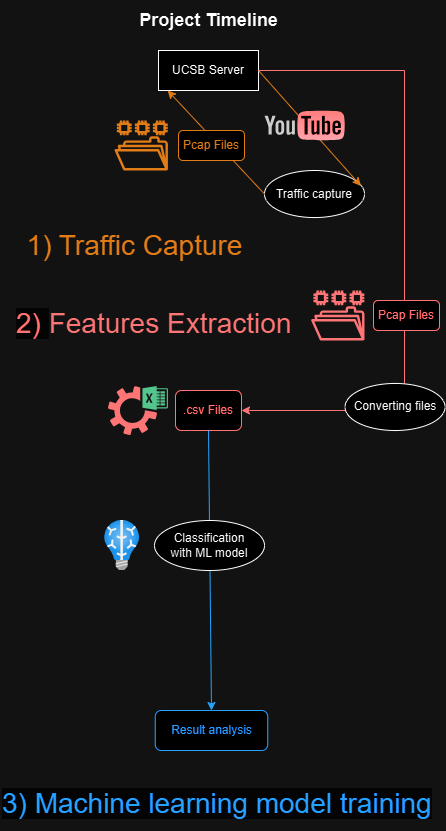
\includegraphics[width=1.0\linewidth]{timeline_diagram.png}
    \label{fig:your_label}
\end{figure}


\hl{Regarding our Machine Learning model, we use a Random Forest model for our classification task. This algorithm processes the input data (that we have previously stored in our .csv files) through an ensemble of decision trees, where each tree and sub-tree analyze and compare different given features, contributing to the final prediction. By combining the outputs of multiple trees, the model generates classifications based on the patterns it has learned during training.
}
\vspace{2mm}

{\hl{The design of our methodology is guided by the following principles:}
\begin{itemize}
    \item \hl{\textbf{Custom Dataset:} By focusing on YouTube traffic and manually selecting videos, we ensure the dataset align with the targeted problem.}
    \item \hl{\textbf{Feature Relevance:} The selected features capture the nuances of gaming and music video traffic.}
    \item \hl{\textbf{Small-Scale Feasibility:} The amount of readily available content on YouTube  makes this project achievable while sticking with a small-scale framework.}
    \item \hl{\textbf{Use of Machine Learning:} Machine learning techniques allow us to overcome the challenges posed by traditional classification approaches and provide flexible solutions for evolving applications.}
\end{itemize}

\hl{This approach provides a strong starting point for and gives us the opportunity to explore and improve further the network traffic classification.}


\begin{algorithm}[t]
\label{algo:tom}
\caption{Sample Algorithm~\cite{sonata}}
\SetKwData{t}{t}
\SetKwData{Empty}{empty}
\SetKwData{Input}{Input}
\SetKwData{Is}{is}\SetKwData{to}{t'}
\SetKwData{E}{$E$}
\SetKwData{In}{in}
\SetKwData{Break}{break}
\SetKwFunction{Extend}{extend}
\SetKwFunction{GRP}{get-refinement-plan}
\SetKwFunction{TOM}{get-tom}
\SetKwFunction{Load}{get-load}
\SetKwFunction{SQ}{sample-queries}
\SetKwFunction{PP}{popular-plans}
\Input: $Q$, $D$\;
$l_{min} \gets \infty$\;
\For{$Th$ $\in [0,M]$}{
$p \gets $ \GRP{$Q$, $Th$, $D$}\;
$l \gets $ \Load{$p$, $D$}\;
% $t \gets $ \TOM{$p$, $D$}\;
% $l \gets 0$; $t \gets 0$\;
% $p \gets $ \GRP{Q', Th, D}\;
% \For{$D_i$ \In D}{
% $t$ $+=$ \TOM{$p$, $D_i$}\;
% $l$ $+=$ \Load{$p$, $D_i$, $\beta$}\;
% }
% $l \gets \frac{l}{|D|}$; $t \gets \frac{t}{|D|}$\;
% \IF{$l$ $\geq$ $l_{min}$}
% {
% \Empty;
% }

% \If{$t \leq \alpha.M$ }

\If{$l \leq l_{min}$ }
{
$l_{min} \gets l$; $p_{min} \gets p$\;
}
% \Else{
% \Break\;
% }
}
\Return $p_{min}$, $l_{min}$

\end{algorithm}
\section{\mbox{Implementation}} \label{sec:implementation}

\begin{algorithm}[H] 
\caption{ML-Based Classification for Gaming and Music Traffic}
\label{algo:ml_pipeline}
\KwData{Network traffic traces (\texttt{.pcap} files)}
\KwResult{Trained Random Forest model, evaluation metrics, predictions, and feature importance}
\BlankLine
\textbf{Step 1: Data Collection}\;
Raw network traffic traces $T \gets$ capture traffic from YouTube videos using \emph{NetUnicorn} pipeline;

\textbf{Step 2: Feature Extraction}\;
$F, L \gets$ extract features from $T$\; \tcp*[r]{Includes Avg Packet Size, Frequency, and Spikes}

\textbf{Step 3: Data Balancing}\;
Apply SMOTE to balance the training dataset\;

\textbf{Step 4: Model Training}\;
Train a Random Forest model on the balanced dataset $(F, L)$\;

\textbf{Step 5: Model Evaluation}\;
Evaluate model performance with metrics: accuracy, precision, recall\;

\textbf{Step 6: Model Prediction}\;
Make predictions on the test set using the trained model\;

\textbf{Step 7: Feature Analysis}\;
Analyze feature importance from the Random Forest model\;

\BlankLine
\Return Trained model, evaluation metrics, predictions, and feature importance\;
\end{algorithm}

\subsection{Data Collection and Traffic Capture}
The first step in our implementation involved capturing network traffic data directly from YouTube. We implemented a pipeline using the \texttt{StartCapture} and \texttt{StopNamedCapture} tasks to log raw network traffic into \texttt{.pcap} files while streaming videos. For each category (gaming and music videos), we processed 18 videos for training and 2 videos for testing, each capturing 100 seconds of data.

To optimize system resources and prevent overload, we introduced a \texttt{SleepTask} between iterations, allowing the system to stabilize. Additionally, we used the \texttt{UploadToWebDav} task to upload captured \texttt{.pcap} files to the central Unicorn server for storage and subsequent analysis.

\subsection{Feature Extraction and Data Processing}
Once the \texttt{.pcap} files were captured, they were converted into \texttt{.csv} files using CICFlowMeter. This tool extracted key numerical features from the raw network traffic, including:
\begin{itemize}
    \item \textbf{Average Packet Size:} The mean size of packets transmitted during the flow.
    \item \textbf{Packet Frequency:} The rate of packets sent during the flow.
    \item \textbf{Forward and Backward Spikes:} The variation in the number of forward and backward packets.
\end{itemize}

We manually combined multiple \texttt{.csv} files into comprehensive datasets for each category (gaming and music). We also added a \texttt{Music} and \texttt{Game} label to the respective data entries to ensure accurate classification.

\subsection{Data Balancing and Preprocessing}
To fix the potential imbalance in the dataset, we applied the SMOTE (Synthetic Minority Oversampling Technique) algorithm to resample the training data. This ensured equal representation of both gaming and music video categories, improving the model's overall stability.

During preprocessing, we calculated additional derived features such as \texttt{Packet Frequency}, \texttt{Forward Spikes}, and \texttt{Backward Spikes}. These features were verified for consistency by analyzing their distributions using histograms and identifying any anomalies or patterns.

\subsection{Model Training and Validation}
A Random Forest classifier was selected for the classification task, leveraging its ability to handle high-dimensional data and provide robust results. We used the \texttt{scikit-learn} library for implementation. 
The model was trained on the resampled dataset with the following features:
\begin{itemize}
    \item \texttt{Avg Packet Size}
    \item \texttt{Packet Frequency}
    \item \texttt{Forward Spike}
    \item \texttt{Backward Spike}
\end{itemize}


\subsection{Fine-Tuning and Feature Importance}
Considering the diversity of features is insufficient on our project-scale to accurately achieve our intended target, we added cross validation adjusted several hyperparameters of the Random Forest model, including the number of estimators, maximum depth, and feature selection techniques. Cross-validation allowed us to train and test the model on different subsets of data, helping us fine-tune it for better performance on unseen data.

Feature importance analysis was conducted to identify which attributes contributed the most to the classification. The Random Forest model indicated that \texttt{Packet Frequency} and \texttt{Data spikes} were the most significant features although they were not sufficient on their own to achieve our intended goal.

To visualize feature importance, we plotted a horizontal bar graph ranking the features by their relative importance, allowing us to understand which aspects of the traffic data were most relevant to the classification task.

\begin{figure}[H]
    \centering
    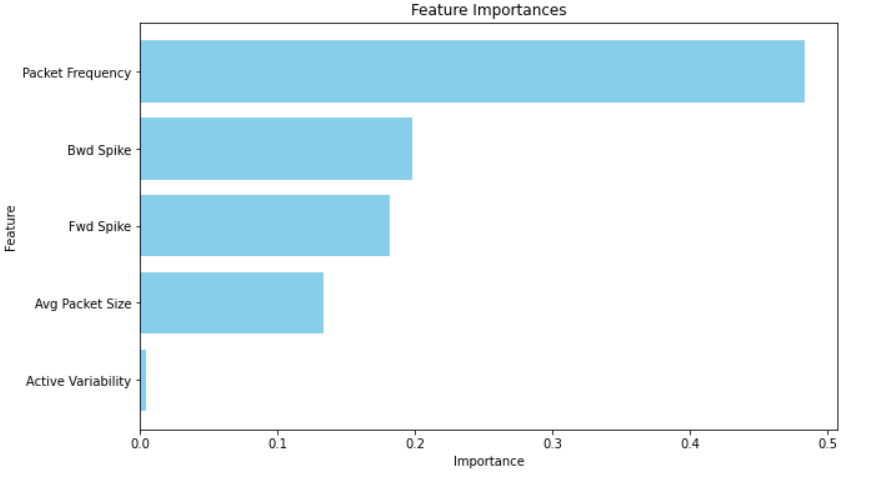
\includegraphics[height=4cm]{features_importance.png} 
    \caption{Feature Importance Analysis}
    \label{fig:features_importance}
\end{figure}


\subsection{Challenges encountered and how we solved them}
Throughout the implementation, several challenges we encountered several challenges:
\begin{itemize}
    \item \textbf{Path Issues:} Automating file handling during the \texttt{.pcap} to \texttt{.csv} conversion resolved errors related to incorrect file paths.
    \item \textbf{Data Imbalance:} Using SMOTE ensured balanced training data, reducing bias in the classification model.
    \item \textbf{Noise in Traffic Data:} Isolating YouTube streams and cleaning the dataset minimized unrelated traffic.
    \item \textbf{Hyperparameter Tuning:} Adjusting hyperparameters helped improve classification accuracy and reduce overfitting.
    \item \textbf{Data Quality Issues:} Removing blank data and refining derived features such as \texttt{Spike Difference} enhanced the consistency of the dataset.
\end{itemize}


\section{Evaluation}
\label{sec:eval}
Below is a good checklist for evaluation.
\begin{itemize}
    \item Appropriate figures of merit to evaluate the work are identified and motivated.
    \item Figures of merit are measured given a comprehensive range of practical parameters / operating conditions.
    \item Experimental setup is described sufficiently for a reader to replicate the testbed.
    \item Conclusions about the core insight of the paper make sense and draw cleanly from the experimental data.
    \item Design decisions are evaluated independently; role of each design choice is backed up with experimental data.
\end{itemize}

In the preamble of your evaluation section, provide a summary of questions that you aim to answer and preview of key results. The first sub-section of evaluation typically describes the setup, which includes description of dataset(s), testbed(s), tools, etc. I highly recommend WALTERing your graphs. 
\begin{itemize}
    \item \textbf{W}hy: why are we looking at this graph
    \item \textbf{A}xes: clearly describe the two axes and measurement units for each
    \item \textbf{L}ines: clearly describe what different lines/shapes represent in the graph
    \item \textbf{T}rends: What clear trends are visible in the graph, what's the implication
    \item \textbf{E}xceptions: clarify if there are some exceptions to the expected trend, explain why
    \item \textbf{R}ecap: provide a takeaway message and try to connect this with the motivation (part of Why).  Are the results as expected? What did we learn from it this experiment?
\end{itemize}

As a rule of thumb, there should only be one main takeaway from a graph. 





\begin{table}[t]
\begin{footnotesize}
\begin{center}
\resizebox{\linewidth}{!}{%
\begin{tabular}{|l| c c  c|}
\hline
\textbf{} & 
\textbf{\begin{tabular}[c]{@{}c@{}}Is\\ Realizable\end{tabular}} &
\textbf{\begin{tabular}[c]{@{}c@{}}Query\\ Planning\end{tabular}} &
\textbf{\begin{tabular}[c]{@{}c@{}}Stream Processor\\ Load\end{tabular}} 
\\

Static-MW  & \cmark & Static & 39.7~M \\ 
\hline
\system-Oracle & \xmark & Dynamic & 37.1~K \\
\system-Pred & \cmark & Dynamic & \textbf{39.6~K} \\
\hline
Optimal-Sonata & \xmark & Dynamic & 21.9~K 
\\ 
\hline
\end{tabular}
}
\end{center}
\end{footnotesize}
% \caption{Query-planning techniques emulated for evaluation.}
\caption{Sample table~\cite{sonata}.
% \ag{TODO: remove refinement column, update the load column.}
}
\label{tab:query_plans} 
\vspace{-.35in}
\end{table}



\begin{figure}[t] 
\begin{minipage}{1\linewidth}
\includegraphics[width=.9\linewidth]{1a.pdf}
\end{minipage}
\caption{Sample figure (results).
\label{fig:cost_of_not_adapting}
}
\end{figure}
% \section{Related Work}\label{sec:related}


%\balance
\section{Conclusion}\label{sec:conclusion}
Make sure that the takeaways are insightful and thoroghly support the key idea/contribution of the work. You can also highlight the limitations of the proposed approach and suggest meaningful future work. 
\label{lastpage}

\end{sloppypar}

\vspace{-0.01in}
%\section*{Acknowledgments}
% Comments for people we need to acknowledge in the final version.
% \noindent \textbf{Acknowledgments.}
% TBD
\pagebreak
\small
%\setlength{\bibsep}{0pt}
\setlength{\parskip}{-1pt}
\setlength{\itemsep}{-1pt}
% \footnotesize % SPACE
\balance
\bibliography{paper, writing/refs}
\bibliographystyle{acm}
%\bibliographystyle{abbrvnat_noaddr} % SPACE
%\theendnotes % ENDNOTES

{% onlyAbstract
}

%\pagebreak
%\input{appendix}

\end{document}

%%%%%%%%%%%%%%%%%%%%  END OF DOCUMENT  %%%%%%%%%%%%%%%%%%%%